\documentclass{report}
\usepackage[utf8]{inputenc}
\usepackage{booktabs}
\usepackage{graphicx}
\usepackage[italian]{babel}
\usepackage{hyperref}
\usepackage[T1]{fontenc}
\usepackage[utf8]{inputenc}
\usepackage[italian]{babel}
\usepackage{eucal,enumitem}
\usepackage{longtable}
\usepackage{amsmath,amssymb,amsthm}
\usepackage{tikz}
\usepackage{cancel} 
\usepackage{multirow}
\usepackage{multicol}
\usepackage{color}
\usepackage{tabto}
\usepackage{fancyhdr}
\usepackage{xltabular}
\usepackage{pdfpages}
\usepackage{longtable}


\begin{document}
    \begin{figure}[htbp!]
        \begin{center}
            
\includegraphics[width=.25\textwidth]{immagini/FedericoII.png}
        \end{center}
    \end{figure}
\begin{center}
    {\scshape\Large\bfseries\center  Progetto Di Basi Di Dati 2022/2023 \\ Sistema Di Gestione Di una galleria geolocalizzata condivisa}
\end{center}
\vfill
    \begin{center}
	Murano\tab								    Monte	\\
	Stefano\tab									Cristian	\\
	N86004383\tab								N86004326 \\
		\begin{center}
			  GIUGNO 2023
		\end{center}			
    \end{center}
    \newpage
    
    \tableofcontents
    
    \chapter{Analisi del Progetto e requisiti individuati}
\section{Obiettivi}
L’obiettivo del progetto descritto in tale documento è di realizzare un sistema informativo per la gestione di collezioni fotografiche geolocalizzate condivise.
\section{Requisisti sui dati}
Il sistema dovrà contenere informazioni relative:
\begin{itemize}
    \item Gli utenti del sistema
        \begin{itemize}
            \item Le credenziali di accesso.
             \item Informazioni Anagrafiche dell’utente
                \begin{itemize}
                    \item Nome dell’utente
                    \item Cognome dell’utente
                \end{itemize}
        \end{itemize}
    \item Le fotografie scattate dagli utenti del sistema
        \begin{itemize}
            \item L’utente Autore della fotografia
            \item la tipologia di dispositivo di scatto
            \item Il luogo in cui avviene lo scatto
        \end{itemize}
    \item I luoghi in cui avvengono scatti
        \begin{itemize}
            \item Coordinate geografiche del luogo
            \item Eventuale nome del luogo
        \end{itemize}
    \item I soggetti immortalati nelle fotografie
        \begin{itemize}
            \item Tipologia di soggetto immortalato
        \end{itemize}
\end{itemize}

\section{Requisiti funzionali}
Ogni utente avrà accesso ad una sua personale schermata Home in cui potrà:
\begin{itemize}
    \item Visualizzare la propria galleria personale
        \begin{itemize}
            \item Aggiungere la foto alla propria galleria personale.
            \item Eliminare foto dalla propria galleria personale.
            \item Filtrare le foto della propria galleria personale per luogo di scatto.
            \item Visualizzare una classifica dei Top 3 luoghi più immortalati dalle foto della galleria.
        \end{itemize}
    \item Partecipare a gallerie condivise con gli altri utenti
        \begin{itemize}
            \item Condividere fotografie personali con altri utenti, attraverso la galleria che hanno in comune.
            \item Rendere private le fotografie personali condivise con gli altri utenti, in
            modo tale da oscurare a tutti i membri della galleria la foto, che una volta resa privata, tornerà ad essere a disposizione per l’utente che ha scattato la foto nella sua galleria personale, ma non sarà presente in galleria condivisa.
            \item Eliminare fotografie dalla propria vista della galleria condivisa, in modo tale che la foto non sia più visibile all’utente che ha eliminato la foto, ma sia visibile a tutti gli altri membri che fanno parte della galleria condivisa.
            \item Filtrare le foto per soggetto immortalato della propria vista della galleria condivisa.
            \item Visualizzare una classifica dei Top 3 luoghi più immortalati delle foto della galleria.
        \end{itemize}
\end{itemize}

\section{Requisiti Aggiuntivi}
\begin{itemize}
    \item Utente: In relazione all’entità utente, nei suoi attributi è presente il Nome, il cognome e password di accesso alla propria area privata.
    \item FOTO: In relazione all’entità foto, nei suoi attributi è presente la data di scatto della foto, la larghezza e la lunghezza della foto.
\end{itemize}
    \chapter{Progettazione concettuale}
    \section{Introduzione}
        \fontsize{15}{14}\selectfont{ In questa sezione verrà introdotta la progettazione concettuale dell'applicativo. Partendo da un primo diagramma di classe in UML. Dal risultato dell'analisi dei requisiti che devono essere soddisfatti si arriverà a uno schema concettuale ristrutturato. Saranno evidenziati i concetti rilevanti ai fini della rappresentazione dei dati e le relazioni che intercorrono tra di esse.}
        
\section{Class Diagram}
    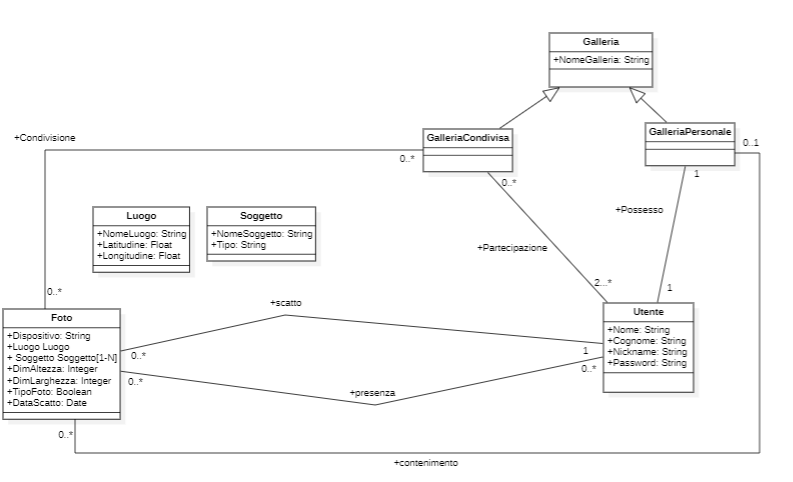
\includegraphics{immagini/MC.png}
        
    \section{Analisi della ristrutturazione del Class Diagram}
        
        \subsection{Analisi delle ridondanze}
            Assenza di ridondanze all'interno del DB
            
        \subsection{Analisi degli identificativi Primari}
            Identificativo dell’entità Utente: Nickname
            \newline
            Inserito un codice identificativo per l’entità foto: CodFoto
            \newline
            Identificativo dell’entità Luogo: NomeLuogo
            \newline
            Inserito un codice identificativo per l’entità soggetto: CodSoggetto
             \newline
            Inserito un codice identificativo della Galleria, ereditato dall’entità 
            figlia GalleriaCondivisa: CodGP
             \newline
            Inserito un codice identificativo della Galleria, ereditato dall’entità figlia GalleriaCondivisa: CodGC
             \newline
        \subsection{Rimozione degli attributi multipli}
            L’attributo Soggetto è stato separato dall’entità di appartenenza Foto e messo in relazione con essa tramite una relazione molti a molti
        \subsection{Rimozione degli attributi composti}
            Gli attributi Luogo e Soggetto sono stati separati dall’entità Foto, andando a formare due nuove entità
        \subsection{Partizione/Accorpamento delle associazioni}
            Non vi sono partizionamenti o accorpamenti delle associazioni
        \subsection{Rimozione delle gerarchie}
        L’entità padre Galleria è stata rimossa e i suoi attributi sono stati ereditati dalle entità figlie Galleria Personale e Galleria Condivisa
\section{Class Diagram ristrutturato}
    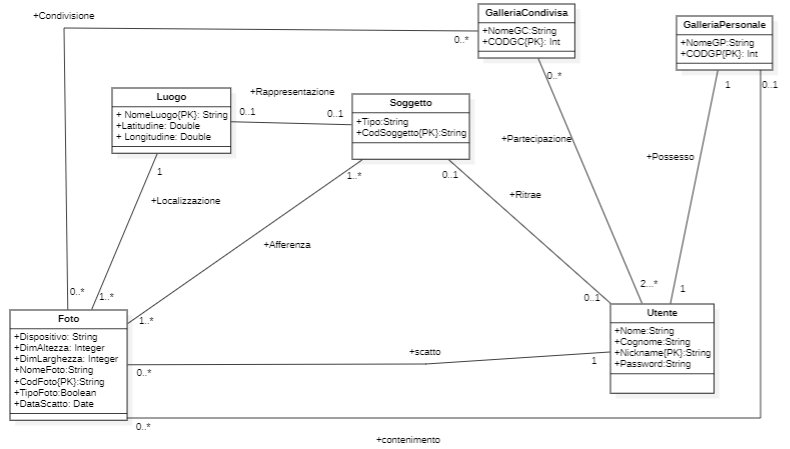
\includegraphics{immagini/MCR.png}

\section{Class Diagram ristrutturato in ER}
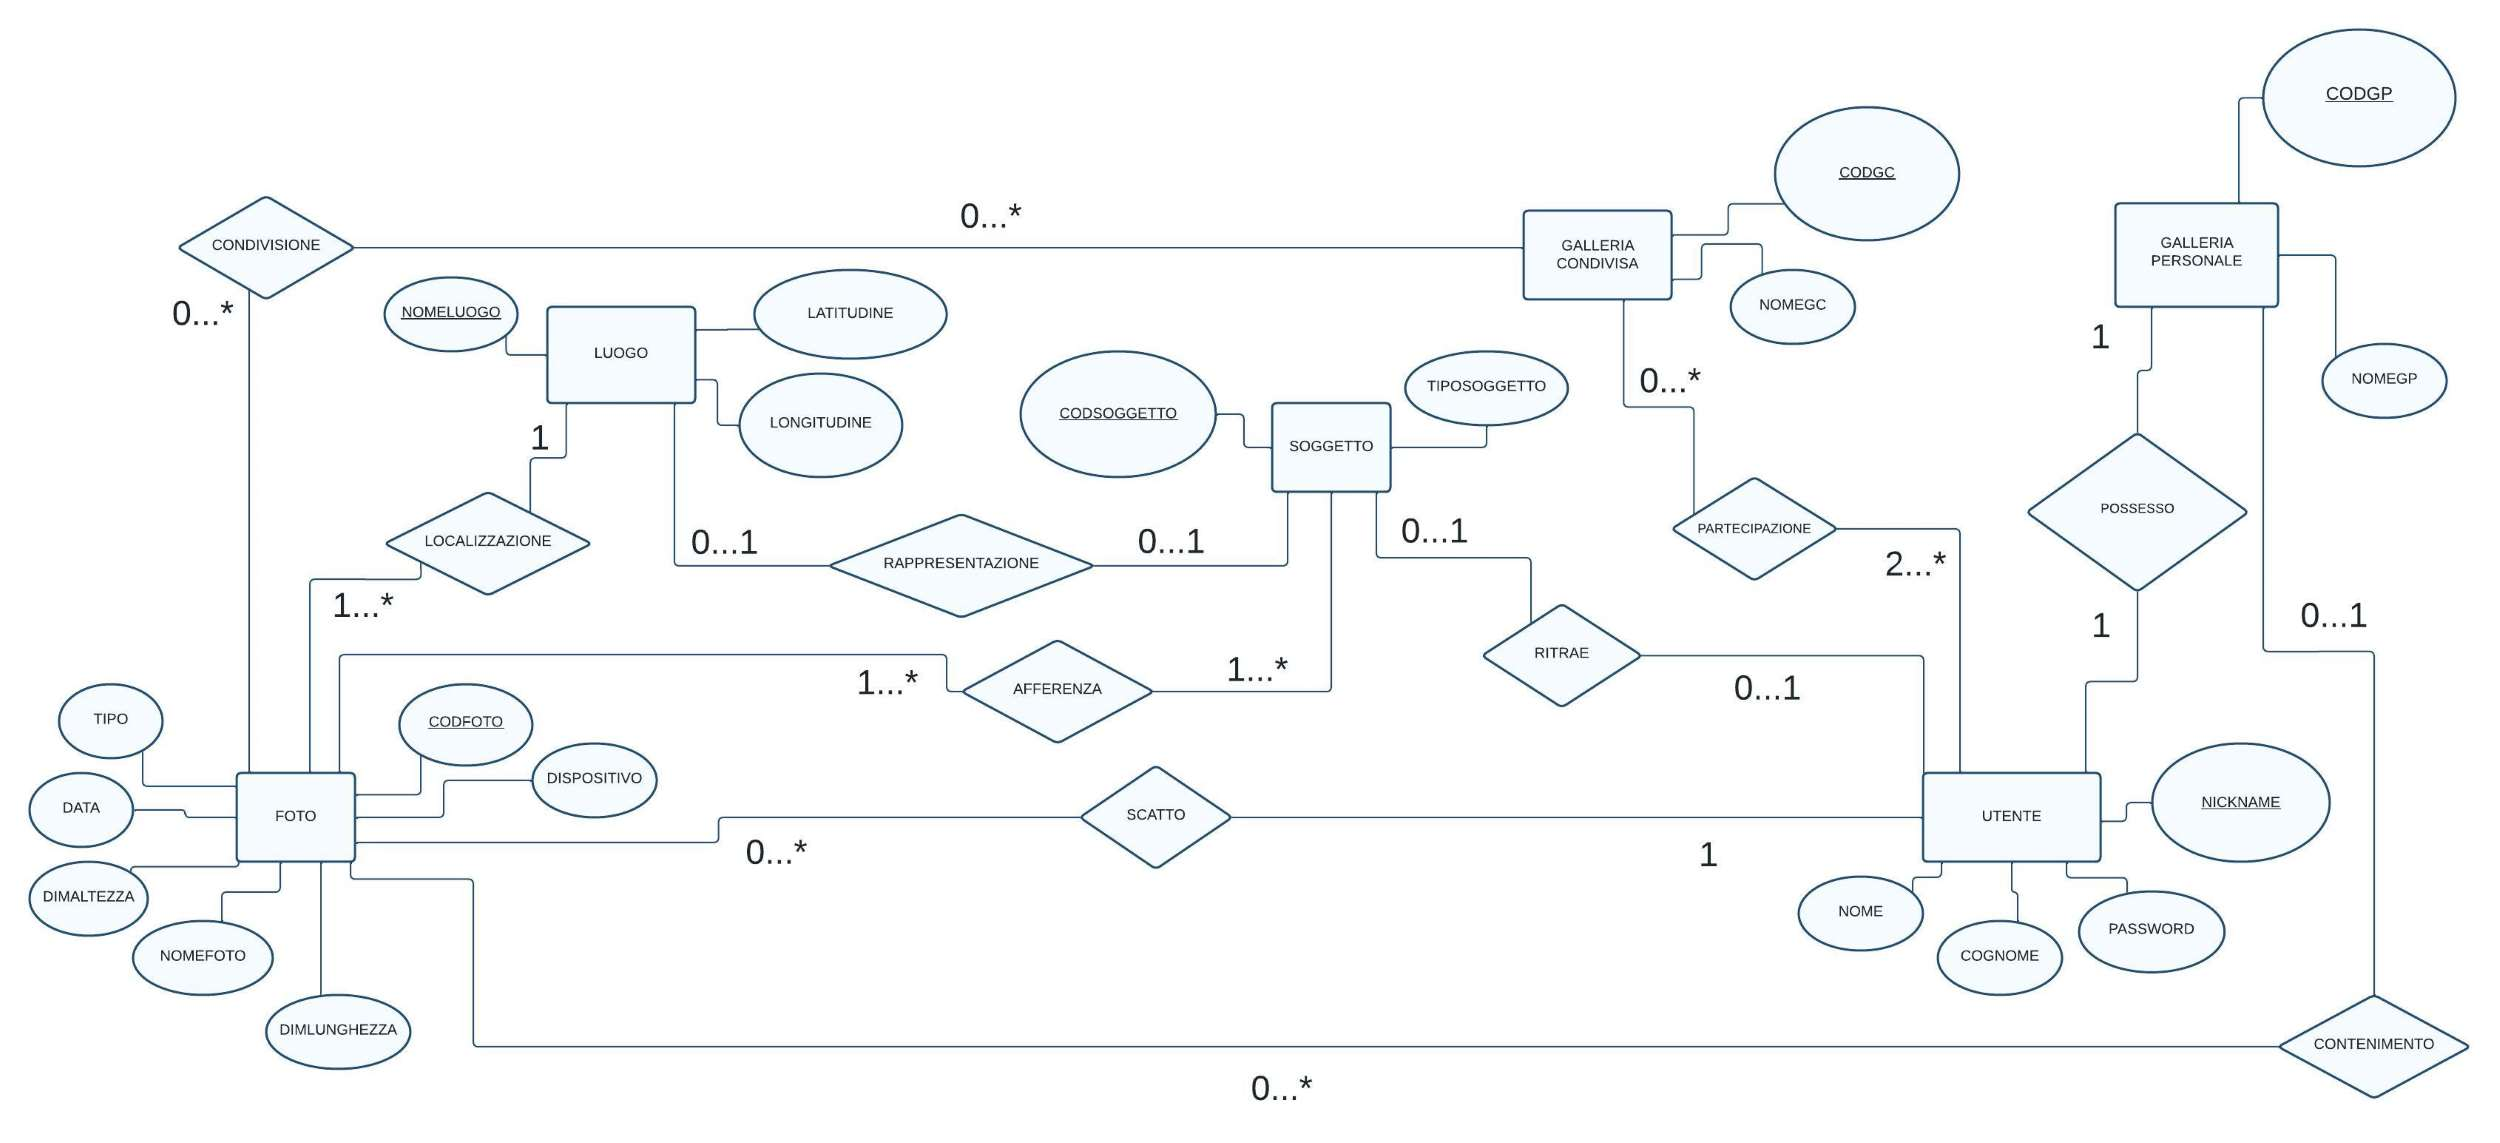
\includegraphics[width=1.4\textwidth]{immagini/Galleria Fotografica Geocalizzata .jpg}
    \chapter{Dizionari}
\section{Introduzione}
\begingroup
        
    \setlength{\tabcolsep}{6pt}
    \renewcommand{\arraystretch}{1.5}
    \begin{xltabular}{\textwidth}{l X X}
        \caption{Dizionario delle classi.} \label{tab:classi} \\

        \hline \multicolumn{1}{|l}{\textbf{Classe}} & \multicolumn{1}{X}{\textbf{Descrizione}} & \multicolumn{1}{X|}{\textbf{Attributi}} \\ \hline 
        \endfirsthead

        \multicolumn{3}{c}%
        {\tablename\ \thetable{} Dizionario delle classi} \\
        \hline \multicolumn{1}{|l}{\textbf{Classe}} & \multicolumn{1}{X}{\textbf{Descrizione}} & \multicolumn{1}{X|}{\textbf{Attributi}} \\ \hline 
        \endhead

        \multicolumn{3}{r}{Continua nella pagina successiva} \\ 
        \hline
        \endfoot

        \hline
        \endlastfoot

        \textbf{Utente} & Entità rappresentante gli individui fruitori del servizio di condivisione di fotografie & \textbf{Nickname} (String): Identificativo univoco dell'utente.
        \newline\textbf{Password} (String): Password di accesso all'area privata dell'utente.
        \newline\textbf{Nome} (String): Nome reale dell'utente.
        \newline\textbf{Cognome} (String): Cognome reale dell'utente.
        \newline\textbf{CodGP} (int): Identificativo univoco della galleria personale dell'utente.\\
        \hline

        \textbf{Galleria Peronale} & Entità rappresentante le gallerie personali degli utenti &     \textbf{CodGP} (int): Identificativo univoco della galleria personale.
        \newline\textbf{NomeGP} (String): Nome assegnato alla galleria personale dal sistema. \\
        \hline

        \textbf{Galleria Condivisa} & Entità rappresentante le gallerie condivise da più utenti & \textbf{CodGC} (int): identificativo univoco della galleria condivisa.
        \newline\textbf{NomeGC} (String): Tipo di Nome assegnato alla galleria condivisa dal sistema.\\
        \hline

        \textbf{Luogo} & Entità rappresentante i luoghi di scatto delle fotografie e i luoghi soggetti delle fotografie & \textbf{NomeLuogo} (String): Identificativo univoco del luogo. 
        \newline\textbf{Latitudine} (Float): Latitudine geografica del luogo. 
        \newline\textbf{Longitudine} (float): Longitudine geografica del luogo. \\
        \hline

        \textbf{Soggetto} & Entità rappresentante i soggetti delle fotografie scattate. & \textbf{CodSoggetto} (String): Identificativo univoco del soggetto.
        \newline\textbf{TipoSoggetto} (String): Tipo associato al soggetto. \\

    \end{xltabular}
\endgroup

\begingroup
        
    \setlength{\tabcolsep}{6pt}
    \renewcommand{\arraystretch}{1.5}
    \begin{xltabular}{\textwidth}{l X X}
        \caption{Dizionario delle classi.} \label{tab:classi} \\

        \hline \multicolumn{1}{|l}{\textbf{Classe}} & \multicolumn{1}{X}{\textbf{Descrizione}} & \multicolumn{1}{X|}{\textbf{Attributi}} \\ \hline 
        \endfirsthead

        \multicolumn{3}{c}%
        {\tablename\ \thetable{} Dizionario delle classi} \\
        \hline \multicolumn{1}{|l}{\textbf{Classe}} & \multicolumn{1}{X}{\textbf{Descrizione}} & \multicolumn{1}{X|}{\textbf{Attributi}} \\ \hline 
        \endhead

        \multicolumn{3}{r}{Continua nella pagina successiva} \\ 
        \hline
        \endfoot

        \hline
        \endlastfoot

         \textbf{Foto} & Entità rappresentante le fotografie scattate dagli utenti. &  \textbf{CodFoto} (int): identificativo univoco della fotografia.
        \newline\textbf{NomeFoto} (String): Nome assegnato alla fotografia dal suo autore.
        \newline\textbf{Dispositivo} (String): Dispositivo di scatto della fotografia.
        \newline\textbf{Nfotografo} (String): Nickname dell'utente, autore dello scatto della foto.
        \newline\textbf{TipoFoto} (Boolean): Grado di visibilità della fotografia che può essere pubblica o privata.
        \newline\textbf{DimLarghezza} (int): Dimensione orizzontale della fotografia. 
        \newline\textbf{DimAltezza} (int): Dimensione verticale della fotografia.
        \newline\textbf{DataScatto} (Date): Data di scatto della fotografia. 
        \newline\textbf{NomeLuogo} (String): Nome del luogo di scatto della fotografia. \\






   \end{xltabular}
\endgroup
\section{Dizionario delle associazioni}

\begingroup
    \setlength{\tabcolsep}{6pt}
    \renewcommand{\arraystretch}{2.0}
    \begin{xltabular}{\textwidth}{l X X}
        \caption{Dizionario delle associazioni.} \label{tab:associazioni} \\
        
        \hline \multicolumn{1}{|l}{\textbf{Nome}} & \multicolumn{1}{X}{\textbf{Descrizione}} & \multicolumn{1}{X|}{\textbf{Classi coinvolte}} \\ \hline 
        \endfirsthead
        
        \multicolumn{3}{c}%
        {\tablename\ \thetable{} Dizionario delle associazioni} \\
        \hline \multicolumn{1}{|l}{\textbf{Nome}} & \multicolumn{1}{X}{\textbf{Descrizione}} & \multicolumn{1}{X|}{\textbf{Classi coinvolte}} \\ \hline 
        \endhead
        
        \multicolumn{3}{r}{{Continua nella pagina successiva}} \\ 
        \hline
        \endfoot
        
        \hline
        \endlastfoot

        \textbf{Rappresentazione} & Esprime la relazione tra Luogo e Soggetto.Un Luogo, oltre ad essere il posto in cui è stata scattata la foto può anche essere il soggetto di una foto. & \textbf{Luogo [0...1]}, indica il luogo associato ad un soggetto in una foto. 
        \newline\textbf{Soggetto [0...1]}, indica il soggetto associato ad un luogo in una foto. \\
        \hline
        \textbf{Afferenza} & Esprime la relazione tra una foto e i suoi soggetti. & \textbf{Foto [1...*]},indica la/le foto a cui partecipa/partecipano uno o più soggetti. 
        \newline\textbf{Soggetto [1...*]},indica il/i soggetto/i che partecipa/partecipano ad una o più foto. \\
        \hline
        \textbf{Ritrae} & Esprime la relazione tra Utente e Soggetto.Un utente, oltre ad essere un fruitore del servizio può anche essere un soggetto della foto. & \textbf{Utente[0...1]},indica l'utente associato ad un soggetto in una foto. 
        \newline\textbf{Soggetto[0...1]},indica il soggetto associato ad un utente. \\
        \hline
        \textbf{Partecipazione} & Esprime la relazione tra Utente e Galleria Condivisa. & \textbf{Utente [2...*]},indica gli utenti che partecipano ad una o più gallerie condivise. 
        \newline\textbf{Galleria Condivisa [0...*]},indica la/le galleria/e a cui partecipa/partecipano 2 o più utenti.\\
        \hline
        \textbf{Condivisione} & Esprime la relazione tra Foto e Galleria Condivisa. & \textbf{Foto [0...*]},indica la/le foto condivisa/e dagli utenti in una o più gallerie condivise. 
        \newline\textbf{Galleria Condivisa [0...*]},indica la/le galleria/e in cui vengono condivise le foto dagli utenti. \\
        \hline
        \textbf{Contenimento} & Esprime la relazione tra Foto e Galleria Personale. & \textbf{Foto [0...*]},indica la/le foto contenuta/e in una galleria personale. 
        \newline\textbf{Galleria Personale [0...1]},indica la galleria in cui è/sono contenuta/e la/le foto personale/i di un utente.\\
        
 \end{xltabular}
\endgroup

\section{Dizionario dei vincoli}

\begingroup
    \setlength{\tabcolsep}{6pt}
    \renewcommand{\arraystretch}{2.0}
    \begin{xltabular}{\textwidth}{l X}
        \caption{Dizionario dei vincoli.} \label{tab:vincoli} \\
        
        \hline \multicolumn{1}{|l}{\textbf{Nome Vincolo}} & \multicolumn{1}{X|}{\textbf{Descrizione}} \\ \hline 
        \endfirsthead
        
        \multicolumn{2}{c}%
        {\tablename\ \thetable{} Dizionario dei vincoli} \\
        \hline \multicolumn{1}{|l}{\textbf{Nome Vincolo}} & \multicolumn{1}{X|}{\textbf{Descrizione}} \\ \hline 
        \endhead
        
        \multicolumn{2}{r}{{Continua nella pagina successiva}} \\ 
        \hline
        \endfoot
        
        \hline
        \endlastfoot

         \textbf{VisibilitaFoto} & Dominio che ha l'utilità di rendere l'attributo TipoFoto boloeano e può essere (pubblico o privato), questo serve a determinare se una foto resta nella galleria privata dell'utente o può essere condivisa. \\

        \textbf{NomeCognomeUtente} & Dominio che ha l'utilità di limitare il tipo di caratteri utilizzabili per descrivere il nome e cognome dell'untente (i caratteri consentiti sono: caratteri alfabetici e spazio). \\

        \textbf{NomeAlfanumerico} & Dominio che ha l'utilità di limitare il tipo di caratteri utilizzabili per descrivere il nickname, password, nomeluogo, nomesoggetto e nomefoto dell'untente (i caratteri consentiti sono: i caratteri alfanumerici, lo spazio, trattino basso e cancelletto). \\

        \textbf{CategoriaSoggetto} & Dominio che ha l'utilità di limitare il range di valori di tiposoggetto ad un insieme di stringhe (luogo, utente, selfie, foto di gruppo, fiera, altro). \\

        \textbf{coordinateluogo} & Rappresenta un vincolo di unicità delle coordinate (latitudine,longitudine) dell'entità luogo. \\

        \textbf{CreazioneGalleriaPersonale} & Vincolo che ha il compito di assegnare ad ogni utente la sua galleria personale. \\

        \textbf{Eliminafoto} & Vincolo che ha il compito di eliminare una foto se non è contenuta in nessuna galleria (sia privata, sia pubblica).\\

        \textbf{RinominaGalleriaCondivisa} & Vincolo che ha il compito di aggiungere al nome della galleria condivisa il rispettivo codice. \\

        \textbf{EliminaLuogo} & Vincolo che ha il compito di eliminare un luogo dall'entità luogo se non è più collegato a nessuna foto(nè come luogo di scatto nè come soggetto). \\

        \textbf{EliminaSoggetto} & Vincolo che ha il compito di eliminare un soggetto dall'entità sogetto, se non è più collegato a nessuna foto. \\
\hline
        \textbf{EliminaSoggettoLibero} & Vincolo che ha il compito di mantenere l'integrità della tabella Soggetto. \\

        \textbf{EliminaLuogoLibero} & Vincolo che ha il compito di mantenere l'integrità della tabella Luogo. \\

        \textbf{EliminaFotoLibera} & Vincolo che il compito di mantenere l'integrità della tabella Foto. \\

        \textbf{EliminaGalleriaVuota} & Vincolo che il compito di mantenere l'integrità della tabella Galleria Condivisa. \\

 \end{xltabular}
\endgroup
    \chapter{Modello Logico}

FOTO(\underline{CodFoto},Dispositivo,DimAltezza,DimLarghezza,\newline\uparrow{NomeLuogo},NomeFoto,TipoFoto, \uparrow{NFotografo})
\newline
FOTO.Nfotografo\leftarrow{UTENTE.Nickname}
\newline
FOTO.NomeLuogo\leftarrow{LUOGO.NomeLuogo}
\newline
\newline
LUOGO(\underline{NomeLuogo},Latitudine, Longitudine)
\newline
\newline
SOGGETTO(\underline{CodSoggetto}, Tipo, \uparrow{NomeSoggetto},\uparrow{NickSoggetto})
\newline
SOGGETTO.NomeSoggetto\leftarrow{LUOGO.NomeLuogo}
\newline
SOGGETTO.NickSoggetto\leftarrow{UTENTE.Nickname}
\newline
\newline
AFFERENZA(\underline{CodFoto, CodSoggetto})
\newline
AFFERENZA.CodFoto\leftarrow{FOTO.CodFoto}
\newline
AFFERENZA.CodSoggetto\leftarrow{SOGGETTO.CodSoggetto}
\newline
\newline
UTENTE(Nome, Cognome,\underline{Nickname},\uparrow{CodGP})
\newline
UTENTE.CodGP\leftarrow{GALLERIA PERSONALE.CodGP}
\newline
\newline
GALLERIA PERSONALE(\underline{CodGP}, NomeGP)
\newline
\newline
GALLERIA CONDIVISA(\underline{CodGC}, NomeGC)
\newline
\newline
PARTECIPAZIONE(\underline{Nickname,CodGC})
\newline
PARTECIPAZIONE.Nickname\leftarrow{UTENTE.Nickname}
\newline
PARTECIPAZIONE.CodGC\leftarrow{GALLERIA CONDIVISA.CodGC}
\newline
\newline
CONDIVISIONE(\underline{CodFoto,CodGC})
\newline
CONDIVISIONE.CodFoto\leftarrow{FOTO.CodFoto}
\newline
CONDIVISIONE.CodGC\leftarrow{GALLERIA CONDIVISA.CodGC}
\newline
\newline
CONTENIMENTO(\underline{CodFoto, CodGP})
\newline
CONTENIMENTO.CodFoto\leftarrow{FOTO.CodFoto}
\newline
CONTENIMENTO.codGP\leftarrow{GalleriaPersonale.CodGP}
\newline

\section{Trigger e Procedure}
Nella seguente sezione vengono riportati tutti i Trigger e le procedure che sono utilizzate nel Data Base relazionale, riportate con il loro nome e la descrizione delle loro operazioni ed utilità.
\newline
\newline
\textbf{CreazioneGalleriaPersonale}: Trigger Function che associa ad ogni nuovo utente, una galleria personale con il nome di "Galleria di Nickname", dove Nickname è il Nickname dell'utente. Utile per avere un uniformità del nome delle gallerie personali.
\newline
\newline
\textbf{RinominaGalleriaCondivisa}:Trigger Function che concatena al nome della galleria condivisa, il corrispettivo codice preceduto dal carattere "Cancelletto".
\newline
\newline
\textbf{CreaElencoUtenti}:Trigger Function che riempie il campo
Elencoutenti della tabella Condivisione. Permette di
condividere una foto in una galleria senza fornirne l’elenco di
partecipanti.
\newline
\newline
\textbf{EliminaUtenteDaElenco}:Procedura che permette ad un
membro di una galleria condivisa di eliminare una foto per sè
lasciandola visibile per gli altri utenti.
\newline
\newline
\newline
\textbf{FiltraFotoPerLuogo}:Funzione che permette di visualizzare tutte
le foto scattate nello stesso luogo.
\newline
\newline
\textbf{FiltraFotoPerSoggetto}:Funzione che permette di visualizzare
tutte le foto che condividono lo stesso soggetto.
\newline
\newline
\textbf{Top3LuoghiPiuImmortalati}:Trigger Function che mantiene
aggiornata la View contenente i 3 luoghi più immortalati in
tutto il database.
\newline
\newline
\textbf{PrivatizzaFoto}:Trigger Function che rimuove una foto resa
privata da tutte le gallerie in cui è condivisa.
\newline
\newline
\textbf{EliminaFotoPrivataGC}:Trigger Function di controllo. Garantisce
che non ci siano foto private in gallerie condivise.
\newline
\newline
\newline
\textbf{EliminaFoto}:Trigger Function che rimuove una foto dal
database se non presente in nessuna galleria, sia personale che
condivisa.
\newline
\newline
\textbf{EliminaLuogo}:Trigger Function che rimuove un luogo dal
database se non associato a nessuna fotografia.
\newline
\newline
\textbf{EliminaSoggetto}:Trigger Function che rimuove un soggetto dal
database se non associato a nessuna fotografia.
\newline
L'utilizzo di tali funzioni (EliminaFoto, EliminaLuogo, ElimanaSoggetto), vengono chiamate ad ogni cancellazione di foto nel database e controllano che i dati relativi alla foto cancellata vengano
correttamente gestiti.
\newline
\newline
\textbf{EliminaFotoLibera}: Trigger Function di controllo. Garantisce che nel database non esistano foto che non sono contenute in alcuna galleria (sia privata e sia condivisa), o che presentino dimensioni errate (una dimensione null ed un'altra not null).
\newline
\newline
\textbf{EliminaSoggettoLibero}:Trigger Function di controllo.
Garantisce che nel database non esistano soggetti che non
afferiscono ad alcuna foto, o che abbiano dati incongruenti (ES. tipo=Utente, NickSoggetto=null).
\newline
\newline
\textbf{EliminaLuogoLibero}: Trigger Function di controllo. Garantisce
che nel database non esistano luoghi che non localizzano o
sono soggetti di alcuna foto o abbiano coordinate errata (una coordinata null ed un'altra not null).
\newline
\newline
\textbf{EliminaGalleriaVuota}:Trigger Function di controllo. Garantisce
che non ci siano gallerie condivise con meno di due partecipanti.
\newline
Le funzioni (EliminaFotoLibera, EliminaSoggettoLibero,
EliminaLuogoLibero, EliminaGalleriaVuota) vengono chiamate
periodicamente e controllano che tutte le foto, soggetti e
luoghi siano consistenti.
\end{document}